This section presents a number of experimental results we obtained to assess multiple facets of the proposed SAR approach. \textbf{(1)} To evaluate the effect of sketching constraints on SAR, as well as, its overall effectiveness in recognizing sketch authorship and detecting sketch fraud, we test SAR on the datasets described in Section \ref{sec:datasets}. \textbf{(2)} We also evaluate the sensitivity of SAR to a number of algorithmic variations. These results, in turn, are used to design the most representative and discriminative variant of SAR. %We believe that this analysis will assist other researchers in developing their own methods for stroke authorship recognition. %\textbf{(3)} To empirically validate the difficulty of the problem at hand, we conduct extensive user studies that establish grounds for comparing human recognition performance to that of SAR.

\vspace{-2mm}
\subsection{Computational Authorship Recognition}\label{subsec:recognition}
\vspace{-2mm}
To answer the questions: Are simple strokes unique to the artist who draws them?  If they are, then to what extent can they identify the author who drew them? To our knowledge, these questions are not adequately addressed in prior work. To answer them, we conduct several experiments on three separate datasets, which provide a rich diversity of sketch content and sketching constraints. In what follows, we report SAR classification accuracy for each dataset and provide cross-dataset analysis. We also evaluate SAR's ability to detect sketch fraud using the fraud dataset.

%\paragraph{Flower Dataset.} This dataset is created by asking 4 artists to draw the same sketch of a flower multiple times without imposing any other instructions or constraints. SAR authorship classification accuracy on test data for this dataset is 96\% and 88\% using leave-one out and 5-fold cross validation respectively with 15\% standard deviation. For comparison, a random choice classifier in this case has an average accuracy of 25\%.

%\paragraph{Character Dataset.} In this dataset, the same character (at 12 different viewpoints) is drawn by 3 different artists. Similar to the flower dataset, artists were given the freedom to draw the cartoon character as they saw fit. SAR accuracy in this case is 87\% (leave-one) and 83\% (5-fold cross validation) with a standard deviation of 12\%. This accuracy is significantly higher than random chance (i.e. 33\%).
%\vspace{-3mm}
\noindent\textbf{Free Style Dataset.} On this constraint-free dataset, SAR accuracy on test data is 60\% and 57\% using leave-one out and 2-fold validation respectively with 8\% standard deviation. For comparison, random chance in this case is 14\%.

%As mentioned earlier, we compiled this dataset by asking 7 different artists to draw 10 different objects that are of various semantic meanings without imposing any other instructions or constraints. SAR authorship classification accuracy on test data for this dataset is 60\% and 57\% using leave-one out and 5-fold cross validation respectively with 8\% standard deviation. For comparison, a random choice classifier in this case has an average accuracy of 14\%.
%\vspace{-3mm}
\noindent\textbf{Fraud Dataset.} Is artistic style among different artists still preserved when they are consciously attempting to commit fraud? To answer this, we use our fraud dataset to build a 7-class SAR classifier to discriminate among the 7 artists. Using this dataset, random chance is 14\%. Here, SAR reaches a significantly higher average accuracy of 51\% (leave-one-out) and 45\% (2-fold cross validation) with 9\% standard deviation. This result suggests that an artist's sketching style is still distinguishable (to a certain extent) even when attempting sketching fraud. To visualize the discrimination power of SAR, we show the BoW features of three sketches (same object) drawn by 3 artists from this dataset in Figure \ref{HistogramsComparisonFraud}. One of the sketches is an original and the rest are fraudulent. Although all three sketches look very similar, their underlying features have obvious differences, which SAR capitalizes on to determine authorship.\\


\vspace{-3mm}
\begin{figure}[!htb]
\centering
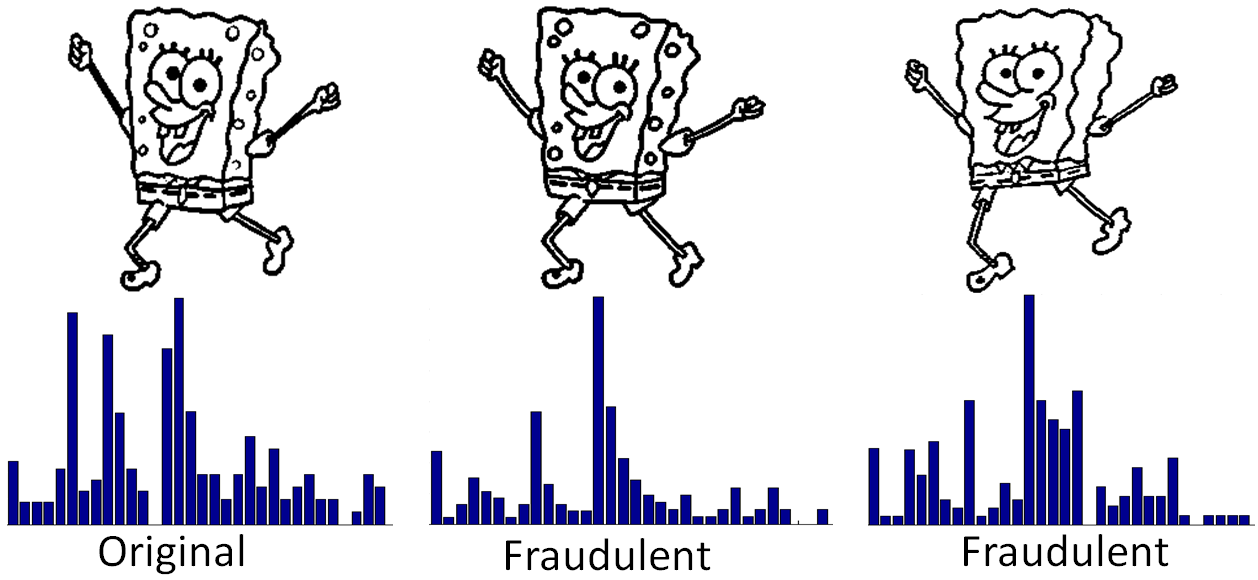
\includegraphics[width = 0.5\textwidth]{images/HistogramsComparisonFraud3.png}
\vspace{-5mm}\caption{BoW features of the same sketch object drawn by 3 artists (one original and two fraudulent). Although they look very similar, their features are different.}
\label{HistogramsComparisonFraud} \vspace{-4mm}
\end{figure}



%in an open case (i.e. the fraudulent identity is not known), which is usually the scenario in reality. For this purpose, we entirely exclude one set of fraudulent sketches by one of the artists from the training samples and used that as our test. For the training part, we have gradually increased the number of fraudulent sketches, starting by 10 sketches and ending with 50 sketches. This is along with the original sketches. Average binary classification accuracy results as the number of training samples increases are shown in Figure \ref{fraudResults}. Results have shown that  the more we train SAR on what is not original, the better its ability gets in detecting an external fraudulent sample to reach up to 96\% classification accuracy when 50 fraduelant sketches are used in the training.  Overall we conclude that espite the extremely high similarity between fraudulent and original sketches, SAR is able to effectively spot fraud. In fact, this sheds light on SAR's applicability and usefulness in the field of artistic fraud detection. \SARA {One could say this is due to the increased probability of detecting the fraudulent sketches with non-balanced binary classes (discuss with Bernard)}

%This dataset has a different setup than the previous ones. A set of 6 artists were asked to simulate an attempt at sketching fraud by drawing a set of sketches labeled as \emph{originals}, which were drawn by a $7^{\text{th}}$ artist. They were specifically instructed to make their own drawings  considerably hard to distinguish from the original ones. This experiment aims to evaluate SAR's ability to detect fraud in a realistic scenario.

%65\% - 73\% - 78\% - 86\% - 96\%
%There are 10 original sketches and 60 fraudulent ones in total, which leads to a substantially unbalanced dataset.

%Special care was taken in training (e.g. dataset downsampling and sample pruning), so as not to artificially bias the SAR classifier to the fraudulent class that contains much more samples than the original class. As a result, SAR successfully detects fraudulent sketches with an accuracy of 95\% (leave-one out) and 92\% (2-fold cross validation) and with a standard deviation of 14\% . Despite the extremely high similarity between fraudulent and original sketches, SAR is able to effectively spot fraud. In fact, this sheds light on SAR's applicability and usefulness in the field of artistic fraud detection.

%Thus, we have 2 groups, one contains the original sketches and the other contains the fraudulent ones and it has much more number of sketches than the ones in the original. To avoid falling into classifying non-balanced data, we randomly selected the same number of sketches as in the original sketches from the pool of fraudulent sketches so that equal classification chances are assigned to test data.


%\vspace{-2mm}
\noindent\textbf{Line Study Dataset.} The sketching task in this dataset (compiled by ~\cite{Cole:2008:PDL:1360612.1360687}) is highly constrained as discussed in Section \ref{sec:datasets}. As it is similar in spirit to the fraud dataset, we expect similar results. We train and test SAR in the same way as before but with a total of 11 artists and 107 sketches. With 11 classes, random chance is 9\%, which is significantly lower than SAR's average accuracy of 33\% (leave-one out) and 30\% (2-fold) with 7\% standard deviation. This noteworthy discrepancy in performance indicates that artists still maintain some uniqueness in their sketching style, even though they are being forced to copy a different style altogether.

We give a performance summary on the three datasets in Table ~\ref{table:accuracy}. The slight difference in accuracy between leave-one out (i.e. all but one sketch are used for training) and 2-fold cross validation (i.e. only 80\% of the sketches are used for training) indicates that SAR is reasonably insensitive to the amount of training data used. This also suggests that SAR is generalizable, a promising property for a classifier in the presence of unseen data.

%\begin{table}[htbp!]
%\caption {A summary of SAR performance on three datasets. Average accuracy is reported for leave-one-out and 2-fold setups. Random chance accuracy and the number of classes are also provided.}
%\label{table:accuracy}
%\vspace{-2mm}
%\centering
%\small
%\begin{tabular}{p{1.1cm} p{0.5cm}  p{0.7cm} p{1.4cm} p{1.0cm} p{0.3cm}  }
%& Num classes & Random Choice \% & Leave-One Out \% & 2-Fold  \% & std \% \\ \hline

%Free Style           & 7 & 14 & 60 & 57 & 8 \\
%Fraud                & 7 & 14 & 51 & 45 & 9\\
%Line Study           & 11& 9  & 33 & 30 & 7\\
%\end{tabular}
%\end{table}

\begin{table}[htbp!]
\caption {A summary of SAR performance on three datasets. Average accuracy \% is reported for leave-one-out and 2-fold setups. Random chance accuracy \% based on the number of classes is also.}
\label{table:accuracy}
\vspace{-2mm}
\centering
\small
\begin{tabular}{cccccc}
&Rand Choice &Leave-one out & 2-Fold &std \\ \hline

Free Style           & 14 & 60 & 57 & 8\\
Fraud                & 14 & 51 & 45 & 9\\
Line Study           & 9  & 33 & 30 & 7\\
\end{tabular}
\end{table}

%\vspace{-2mm}
\noindent\textbf{Cross-Dataset Analysis.} In the datasets above, the contributing artists were subject to varying levels of sketching constraints, ranging from unconstrained (free style dataset) to highly constrained (line study dataset). To investigate the sensitivity of SAR performance with sketching constraints, we compare its accuracy across all datasets in Figure ~\ref{crossDatasetsPlot}. The datasets are ordered in increasing levels of constraint. To normalize the effect of different numbers of classes across datasets, we plot the ratio of SAR accuracy to random chance. As expected, recognizing sketch authorship becomes harder as more constraints are imposed on the artist. However, on all the datasets, SAR performance is significantly (at least 2.5 times) higher than random chance. This suggests that artists do \emph{not} lose all characteristics of their unique style even under the strictest of constraints.

%a comparison between SAR performance across all datasets, so as to investigate how the uniqueness of artistic strokes is influenced by imposing more control and adding more constraints on the sketching process. In Figure ~\ref{crossDatasetsPlot}, datasets are ordered in increasing amount of constraint. As might be expected, the recognition performance (w.r.t. to random chance) is inversely proportional to the amount of constraints imposed. From this experiment, we are lead to two main conclusions. First, the more freedom artists are given during the sketching process, the more likely their unique artistic style will be preserved. Second, even with highly constrained sketching tasks such as sketching fraud, artistic strokes maintain a certain level of uniqueness and discriminability.

\begin{figure}[htbp!]
\centering
\subfigure[]{
  \centering
  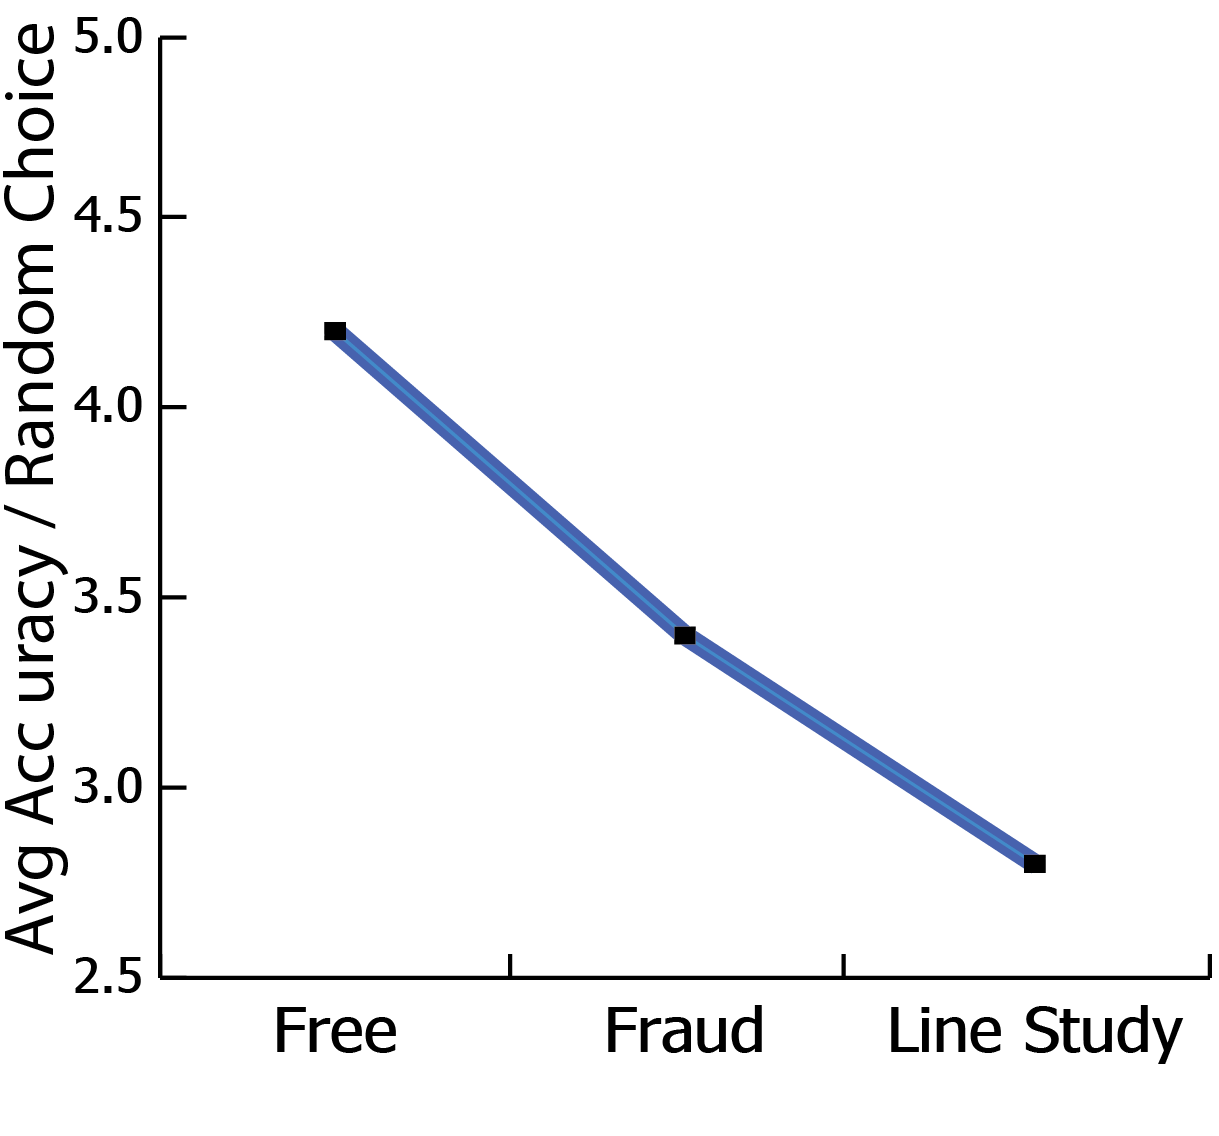
\includegraphics[width=0.225\textwidth]{images/sketchConstraints.png}
  \label {crossDatasetsPlot}
}\hspace{-3mm}
\subfigure[]{
  \centering
  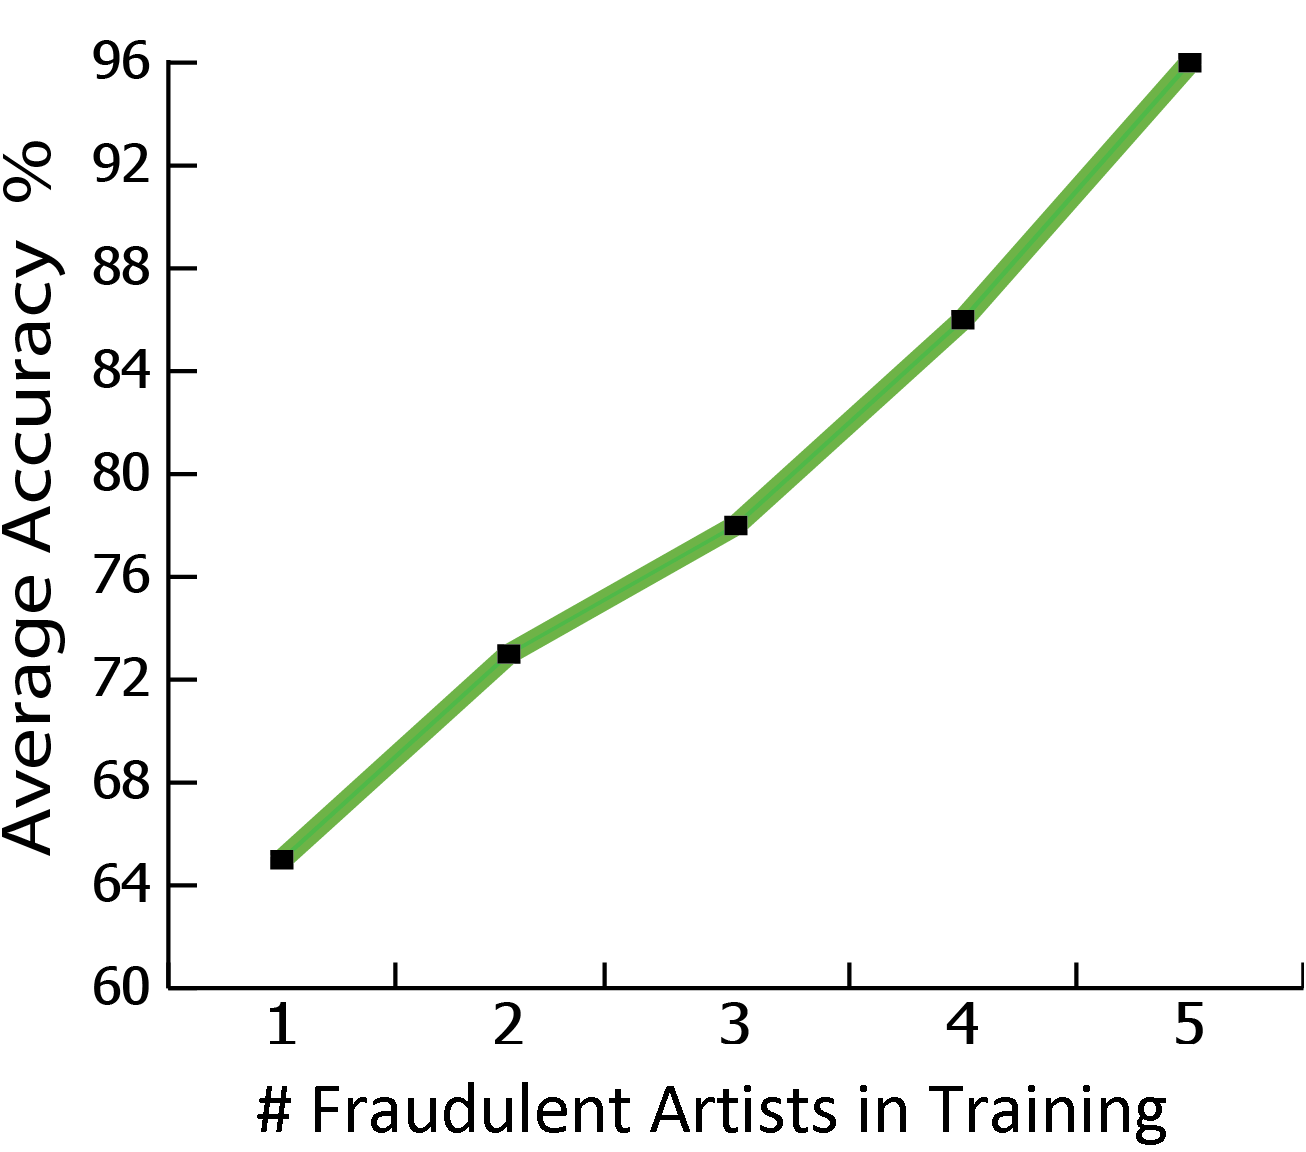
\includegraphics[width=0.225\textwidth]{images/fraudResults.png}
  \label {fraudResults}
}
\vspace{-2mm}\caption{(a) The ratio between SAR accuracy and random chance on three datasets organized in increasing order of sketching constraints. Clearly, the more constraints imposed on artists, the less discriminative their strokes become. (b) Fraud recognition performance improves as more fraudulent artists are used in training, especially on sketches from artists who were not included in training.}\vspace{-3mm}
\end{figure}


\begin{figure*}[htbp!]
\centering
\subfigure[]{
  \centering
  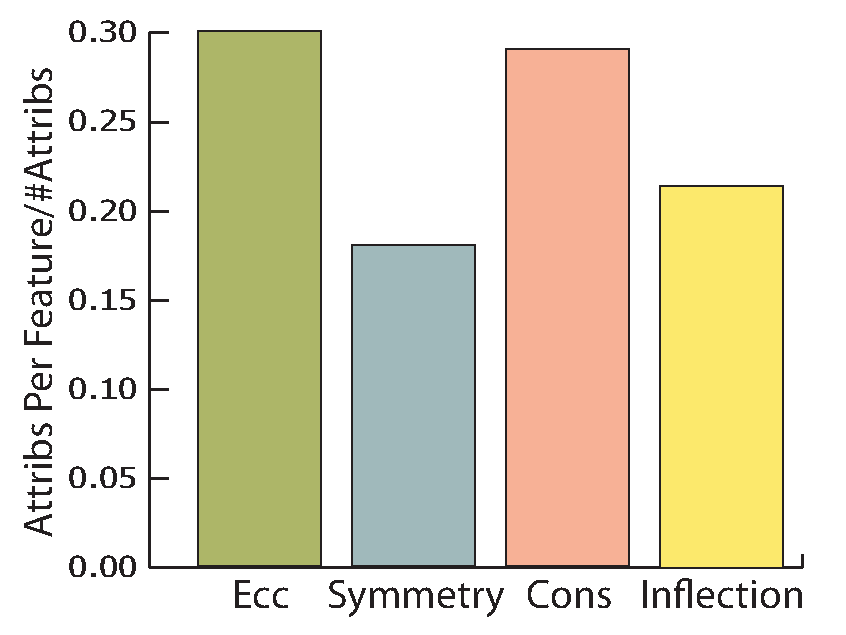
\includegraphics[width=0.35\textwidth]{images/FeatureTypeCont}
  \label {FeatureTypeCont}
}
\subfigure[]{
  \centering
  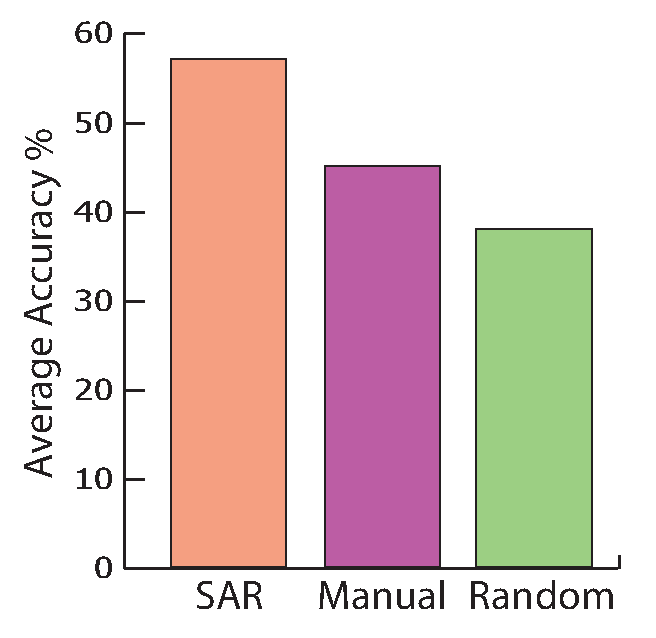
\includegraphics[width=0.27\textwidth]{images/segAlg}
  \label {segAlg}
}
\subfigure[]{
  \centering
  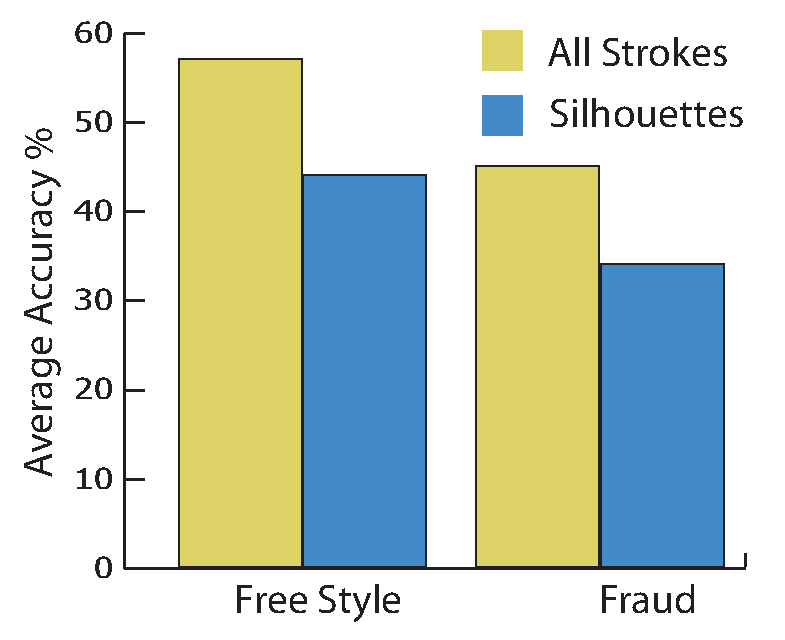
\includegraphics[width=0.32\textwidth]{images/sillVsInternal}
  \label {silAssesPlot}
}
\vspace{-4mm}\caption{(a) Contribution of each feature type to SAR recognition. (b) SAR accuracy on the free style dataset when its segmentation method is replaced with a manual or random one. SAR outperforms manual segmentation by around 15\% and random segmentation by around 20\%. (c) SAR accuracy on the free style dataset, where stroke segments come from the silhouette only or from the entire sketch. Adding internal stroke segments \emph{does} improve accuracy but the improvement is only about 10\%.}\vspace{-4mm}
\end{figure*}
%\begin{figure}[ht]
%  \centering
%  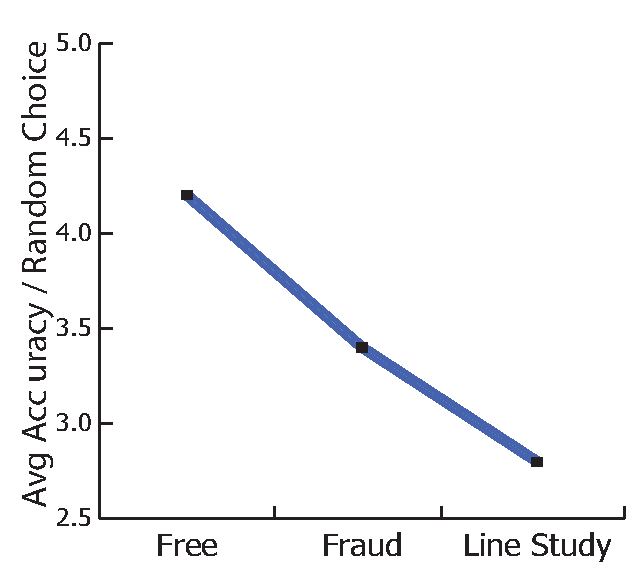
\includegraphics[width=0.42\textwidth]{images/sketchConstraints}
%  \caption{A plot of the ratio between SAR accuracy and random chance on all the datasets included in this paper. The datasets are organized on the horizontal axis in the order of increasing amount of sketch constraints. We see that the more constraints are added to how artists sketch, the less discriminative their strokes become.}
%  \label{crossDatasetsPlot}
%\end{figure}

%\vspace{-2mm}
\noindent\textbf{Fraud Recognition Experiment.} Here, we setup a fraud recognition experiment (original vs. fraudulent) that predicts SAR performance in a real-world scenario. It is unrealistic to assume that the SAR classifier will have access to fraudulent training examples from \emph{all} artists. However, we expect that when more fraudulent samples are used in training, SAR's test performance on fraudulent sketches from artists, who were \emph{not} included in training, will improve. In other words, knowing more about how fraud \emph{looks} like will help SAR better detect sketch fraud, even for fraudulent artists whose sketches are not trained on. To validate this expectation, we train the SAR binary (fraud vs. original) classifier with fraudulent sketches from increasingly more fraudulent artists (i.e. from 1 to 5 artists). In each case, 80\% of the original sketches are used for training (2-fold validation). Then, each SAR classifier is tested on the remaining original and fraudulent sketches. This means that SAR will always be tested on fraudulent sketches from artists, whose style has not been seen during training. In Figure \ref{fraudResults}, we plot the average test accuracy of SAR as the number of fraudulent artists used in training increases. Clearly, this result endorses our aforementioned expectation. In fact, SAR's fraud detection performance reaches 96\% when 5 of the 6 fraudulent artists are used for training and the $6^{\text{th}}$ for testing. Despite the extremely high similarity between fraudulent and original sketches, we conclude that SAR is able to effectively spot artistic fraud. In fact, this result suggests that SAR can be useful in an online learning setup, where test samples are sequentially classified and in turn weighted and then used in re-training the classifier. %Our results show that SAR performance would tend to increase with more in this scenario.

%can be very useful in finding sketch fraud (e.g. from online sources), whereby its performance can improve when it adds

%This sheds light on SAR's applicability to the field of artistic fraud detection.

%\begin{figure}[ht]
%\centering
%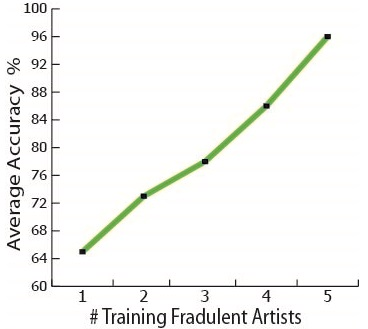
\includegraphics[width = 0.4\textwidth]{images/fraudResults}
%\caption {Fraud detection performance improves as more fraudulent artists are used in training even though testing is done entirely on sketches from fraudulent artists that are not included in training.}
%\label{fraudResults}
%\end{figure}

%SAR is able to estimate how \emph{close} artists-in-training are to a particular style.
%For fair comparison, we use the same number of classes across all datasets.
\vspace{-2mm}
\subsection{Algorithmic Details} \label{subsec:variations}
\vspace{-2mm}
Since SAR comprises multiple computational modules (refer to Figure \ref{pipeline}), varying the details of any module can lead to a variant of SAR. In this section, we investigate many of these variations and provide algorithmic details to reproduce the SAR classifier.

%a number of algorithmic variations, which we experimented with during the development of SAR in order to build the best possible computational model. %We include the following experiments and results with the aim to help others in the community in conducting similar research. %We also assess assessment of some of the techniques used in SAR by comparing them against different techniques.

%\vspace{-2mm}
\noindent\textbf{Feature Contribution.} Stroke segments are represented by 4 biologically inspired features, as discussed in Section \ref{subsec: featureExtraction}. Here, we study the contribution of each feature to SAR's discriminative power. To do this, we employ a conventional forward feature selection method that greedily determines which features (along with their importance weights) should be incorporated into the SAR classifier. This is a data-driven process, so different training-test splits of the dataset can lead to different feature selections and weights. By training SAR (with 2-fold validation) multiple times on the free style dataset, we accumulate an average selection weight for each feature (refer to Figure \ref{FeatureTypeCont}). We see that eccentricity and local consistency are the most discriminative features followed by inflection and symmetry, where no one feature seems to dominate.

%It is obvious that for a feature type to be considered, it must have contributed for better authorship classification accuracy. However, in this section we show the contribution of each feature type as reflected by the number of attributes selected from each feature type using our feature selection algorithm. As shown in , both Eccentricity and Local Consistency have almost the same number of significant attributes followed by Inflection and finally Symmetry. Overall, all feature types have significant attributes in them and the differences between the number of selected attributes between  different features is not large.
%\begin{figure}[ht]
%  \centering
%  \includegraphics[width=0.3\textwidth]{}
%  \caption{The contribution of each feature type}
%  \label{}
%\end{figure}

%\vspace{-3mm}
\noindent\textbf{Variations in Stroke Segmentation.} To justify our stroke segmentation method (refer to Section \ref{subsec:segmentation}, we compare it against two baseline methods: manual and random stroke segmentation.
For manual segmentation, we asked 10 artists to manually segment sketches into strokes as they see fit, while in the random case, breakpoints are selected uniformly at random within each extracted stroke. We set a minimum length for each stroke segment to prevent singularities. SAR accuracy (2-fold) using each of the three segmentation methods on the free style dataset is summarized in Figure~\ref{segAlg}. Clearly, our automated segmentation method outperforms the other two. Similar to the human recognition result in Section \ref{sec:humanexps}, SAR improvement over manual segmentation suggests that human performance on a fine-grained classification task such as authorship recognition does not seem optimal.

%We compared the performance of our segmentation technique against manual and random segmentation methods by running the classification model using the three techniques and check the classification accuracy obtained. For manual segmentation, we manually attempted to segment the strokes at singular and inflection points while in random segmentation we segmented the strokes such that each segment is of a certain number of pixels chosen randomly. Comparison results are shown in ~\ref{segAlg} and it proves that our segmentation technique results in better classification accuracy and thus it is better in detecting a particular artist's sketching style when compared with manual and random segmentation methods.

%\begin{figure}[ht]
%  \centering
%  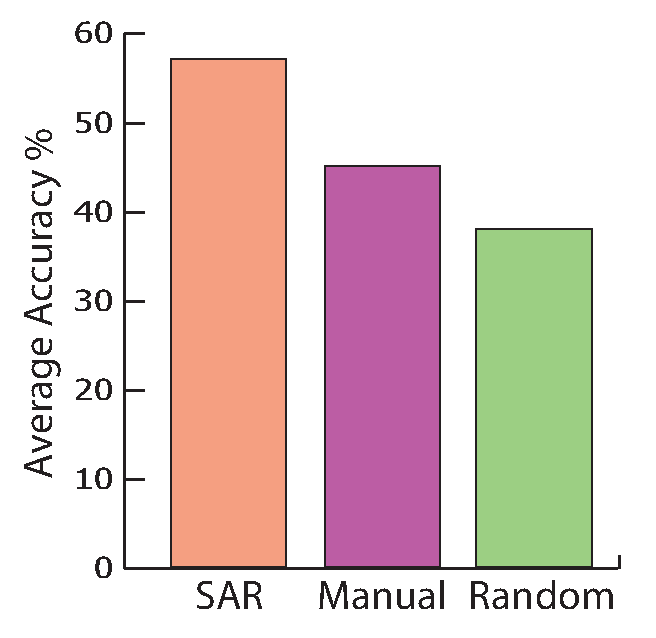
\includegraphics[width=0.3\textwidth]{images/segAlg}
%  \caption{SAR accuracy on the free drawing dataset when its segmentation method is replaced with a manual or random one. The inherent segmentation in SAR outperforms manual segmentation by around 15\% and random segmentation by around 20\%.}
%  \label{segAlg}
%\end{figure}

%\vspace{-3mm}
\noindent\textbf{Silhouettes vs. All Strokes.} In many cases (e.g. the Mickey Mouse cartoon character), the silhouette of a sketch can be very discriminative, so much so, that silhouettes have been used as primary features in other recognition tasks (e.g. action recognition \cite{li2008expandable}). Here, we study how discriminative silhouette stroke segments are on their own within the SAR pipeline. In Figure ~\ref{silAssesPlot}, we use two datasets to compare SAR accuracy when stroke segments are taken from the silhouette alone or from the entire sketch. Interestingly, silhouettes seem to be quite discriminative in their own right, as SAR performance remains high even when only silhouettes are used. In fact, including stroke segments from the sketch interior only improves accuracy by about 10\%.

%is only improved by about 13\% when internal stroke segments are added to silhouette stroke segments. This is a strong indication of the importance of silhouettes in determining sketch authorship.


%it is commonly understood that silhouettes \emph{alone} can contribute very rich information, so much so, that they have been used as primary features in other recognition tasks (e.g. action recognition \cite{silhaction}) \B{missing ref}. In fact, many objects and shapes (e.g. the Mickey Mouse cartoon character) can generally be recognized when just their silhouettes are shown.

%For the task of authorship recognition, we study how discriminative silhouette stroke segments are by themselves.  As shown Figure ~\ref{silAssesPlot}, SAR accuracy on the character dataset is only improved by about 13\% when internal stroke segments are added to silhouette stroke segments. This is a strong indication of the importance of silhouettes in determining sketch authorship.

%including the internal strokes to the silhouettes have just contributed around 10\% to the average classification accuracy and this gives a strong indication of the importance of silhouettes strokes in comparison with all the strokes when used to classify sketch authorship.

%The reason we gave the silhouettes this attention and follow that division is because they contribute a large portion of the entire sketch. Moreover, objects and shapes can generally be recognized when showing just their silhouettes. For example, a famous cartoon character like Mickey Mouse can be easily recognized from its silhouettes and one can recognize a sketch of an object like a table or a pen also by looking at their boundary. Thus, we assumed that silhouettes strokes can play a key factor in recognizing authorship among similar sketches as well.  As can be seen in ~\ref{silAssesPlot}, including the internal strokes to the silhouettes have just contributed around 10\% to the average classification accuracy and this gives a strong indication of the importance of silhouettes strokes in comparison with all the strokes when used to classify sketch authorship.

%\begin{figure}[ht]
%  \centering
%  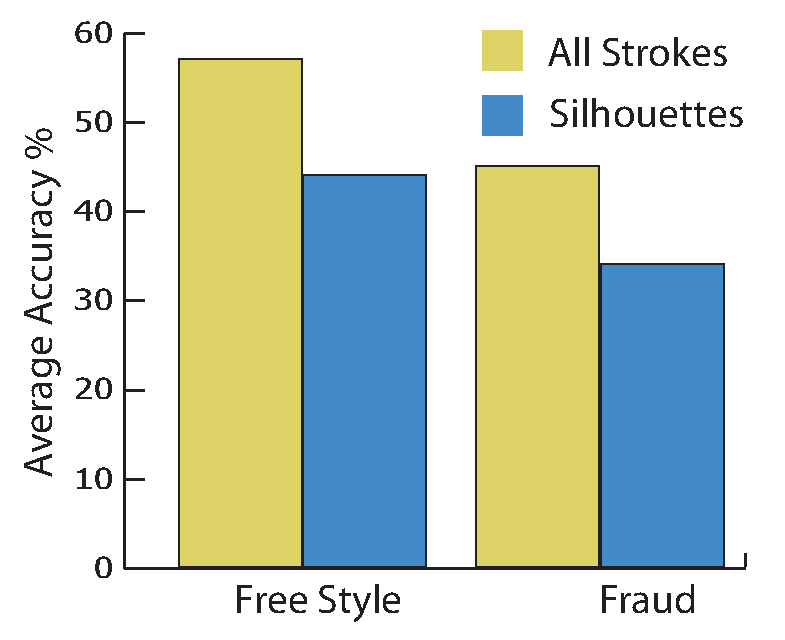
\includegraphics[width=0.3\textwidth]{images/sillVsInternal}
%  \caption{SAR accuracy on 3 sketch datasets where stroke segments come from either %silhouettes only or from the entire sketch. Adding internal stroke segments %\emph{does} improve accuracy but the improvement does not exceed 10\% across all %datasets.}
%  \label{silAssesPlot}
%\end{figure}


%\vspace{-3mm}
\noindent\textbf{Effects of Digitization.} As mentioned in Section \ref{subsec: segmentation}, stroke segments are extracted from a sketch using the well-known Adobe Live Trace digitization technique. The level of digitization is controlled by the user to tradeoff faithfulness to the original sketch with compactness of representation. For instance, high levels of digitization tend to smooth out strokes, thus, masking aspects of the artist's intrinsic style and possibly affecting SAR performance. To investigate the effect of digitization on SAR, it is applied to the fraud dataset after applying three distinct levels of digitization on its sketches. We report the average accuracies in Table \ref{table:digitization}. As expected, the higher the digitization level), the lower the SAR accuracy is. In fact, the accuracy reduces significantly and reaches near random chance when the highest level of digitization is used. This result suggests another application that could benefit from SAR, namely the quantitative assessment of various digitization techniques. SAR can conceivably be used to evaluate how much of the unique sketching style is preserved after digitization.

%digitized sketches to the and evaluate them based on how the artistic style is preserved after digitization.

%In order to be able to extract all the strokes of a given sketch, we use Adobe Live Trace digitization technique which changes a bitmap image into vector. By tracing a sketch, a digitized version is created and Adobe users can control the level of detail and how the tracing is filled. One concern we had was; would the digitization had an influence on the artistic style such that recognition of a sketch authorship is disturbed? We asked this question after noticing that some of the artists' strokes details were smoothed out in the digitized version. With the aim to verify this, we ran SAR on three different sets of silhouettes strokes using the entire Fraud Experiment dataset discussed earlier. First, we applied SAR on the original silhouettes of the sketches. Next, we compared the obtained classification accuracy against 2 different types of the digitized silhouettes created using 2 digitization levels from the Adobe Live Trace options. The first level of digitization uses the best and the tightest approximation to the bitmap sketch while the second level uses the least tight approximation i.e. the resulted silhouettes are very smoothed out. The experiment results showed that the best classification accuracy is obtained by using the non-digitized sketches, then the tightly digitized sketches and finally the loosely digitized sketches as shown in ~\ref{table:digitization}. This indicates that digitization influences the artistic style and encourages the need of digitization techniques that can preserve the artist's unique strokes as best as possible. This also spots the light on one of the useful uses of SAR as it can be used to compare and assess different digitization techniques and evaluate them based on how the artistic style is preserved after digitization.

\vspace{-1mm}
\begin{table}[!htbp]
\caption {Effects of digitization on SAR accuracy \%. Sketches from the free style dataset are processed using three levels of digitization in Adobe Live Trace. SAR accuracy decreases significantly with higher levels of digitization.}
\label{table:digitization}
\vspace{-2mm}
\centering
\small
\begin{tabular}{c | c | c}
level of digitization& leave-one-out & 2-fold cross validation \\ \hline

%Original Sketch         & 48 &  45\\
Low       & \textbf{51} &  \textbf{45}\\
Medium       & 42 &  39\\
High      & 28 &  23\\
\end{tabular}\vspace{-2mm}
\end{table}


%\vspace{-3mm}
\noindent\textbf{Style not Content.} SAR is designed to represent and classify artistic sketch style, irrespective of sketch content in general. This is a primary factor that distinguishes SAR from existing shape matching techniques discussed earlier in Section \ref{subsec: shapematching}. In fact, our experiments show that sketches of different content (objects) drawn by the same artist tend to have more similar BoW features than sketches of the same content drawn by different artists. For instance, the BoW feature of a flower drawn by one artist is more similar to a butterfly drawn by that artist than the feature of the same flower drawn by another artist, as illustrated in Figure \ref{styleVsContent}. To quantify this observation, we use a normalized Gaussian similarity measure $s(\mathbf{I}_1,\mathbf{I}_2)$ based on the Euclidean distance between two BoW features. From the free style dataset, we randomly select a sketch $\mathbf{I}_i^A$ drawn by artist A and the same sketch $\mathbf{I}_i^B$  drawn by another artist B to compute $s(\mathbf{I}_i^A,\mathbf{I}_i^B)$. We then randomly select a sketch $\mathbf{I}_j^A$ drawn by A with $i\neq j$ and compute $s(\mathbf{I}_i^A,\mathbf{I}_j^A)$. By performing this operation across the whole dataset, we compute the average inter-artist similarity $s(\mathbf{I}_i^A,\mathbf{I}_i^B)=68\%$ and the average intra-artist similarity $s(\mathbf{I}_i^A,\mathbf{I}_j^A)=89\%$.  This result shows that SAR targets an artist's style by abstracting it from sketch content.



%we randomly select a sketch drawn by one artist and use the euclidean distance as the similarity metric i.e. less euclidean distance implies more similar histograms. We then picked the same sketch object drawn by 2 other randomly selected artists. Results have shown that a sketch drawn by Artist A is 89\% similar to sketches drawn by the same artist while only 75\% and 68\% similar to the same sketch object drawn by artists B and C.

%Using the free style dataset, we randomly picked a sketch drawn by one artist and use the euclidean distance as the similarity metric i.e. less euclidean distance implies more similar histograms. We then picked the same sketch object drawn by 2 other randomly selected artists. Results have shown that a sketch drawn by Artist A is 89\% similar to sketches drawn by the same artist while only 75\% and 68\% similar to the same sketch object drawn by artists B and C.

%In this section we emphasize that our proposed authorship technique (SAR) provides an artistic style discrimination with no dependency on the sketching content. This is one of the factors that distinguishes SAR from existing shape matching techniques as discussed earlier in Section \ref{subsec: shapematching}.

%We show that various sketches of different objects sketched by one artist tend to have more similar histograms when compared against other sketches of the same content but drawn by another artist. In other words, a flower drawn by one artist has a representing histogram that is more similar to a butterfly drawn by that artist than the histogram of the same flower object drawn by another artist. Using the free style dataset, we randomly picked a sketch drawn by one artist and use the euclidean distance as the similarity metric i.e. less euclidean distance implies more similar histograms. We then picked the same sketch object drawn by 2 other randomly selected artists. Results have shown that a sketch drawn by Artist A is 89\% similar to sketches drawn by the same artist while only 75\% and 68\% similar to the same sketch object drawn by artists B and C.

%as illustrated in Figure ~\ref{styleVsContent}.

\begin{figure}[ht]
  \centering
  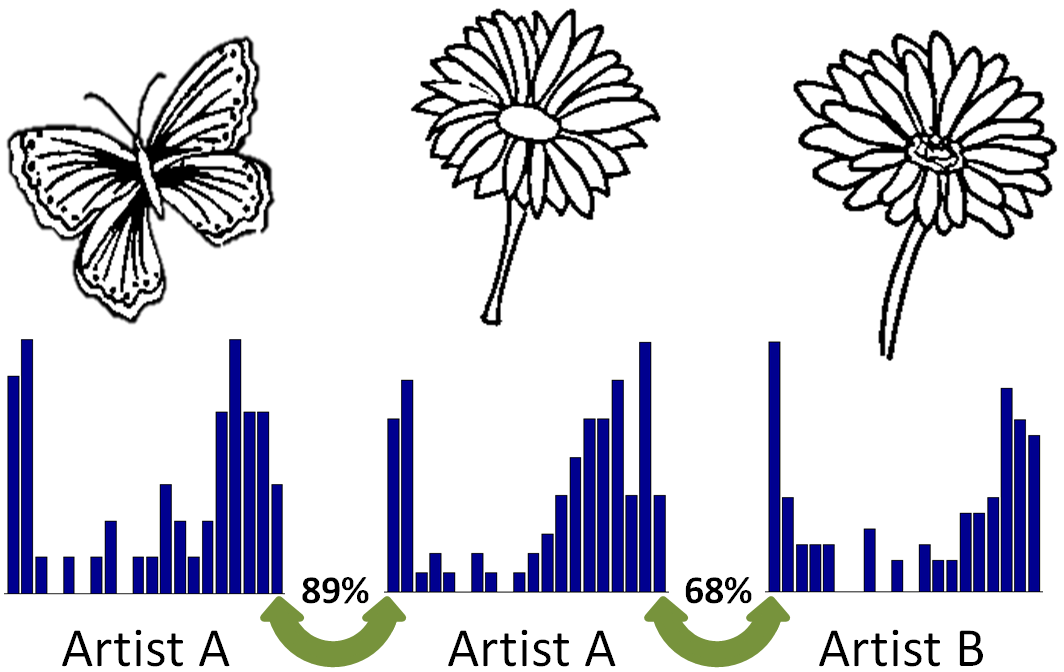
\includegraphics[width=0.5\textwidth]{images/styleVsContent2.png}
  \caption{A visual comparison between the BoW features of three sketches from the free-style dataset: a flower drawn by Artist A (middle), a butterfly drawn by Artist A (left), and the same flower object drawn by Artist B (right). From the features themselves and their average pairwise similarity scores, we see that SAR discrimination is based on artistic style and not sketching content.}
  \label{styleVsContent}
\end{figure}


\iffalse
\subsection{Human Vs. SAR.}
In this section, we summarize the difference in recognition performance between human subjects and our SAR automated system.

we compare human performance against our authorship recognition computational model. The first user study was built using the free style sketching dataset and our user study shows that people can successfully recognize the authorship of a sketch among 7 different artists with an average accuracy of 36\% and with a standard deviation of 10\%, using a sample of more than 2000 participants. SAR, on the hand, recorded an accuracy of 60\% and a standard deviation of 8\% when applied to the same dataset and using the same setup as in the user study. We also conducted another user study which involved 25 artists and using the fraud experiment datase. Artists were asked to distinguish fraudulent and original sketches using samples of both. User study results showed that given a set of sample sketches, artists can distinguish between fraudulent and original sketches with an average accuracy of 52\% and a standard deviation of 10\% while SAR classified fraudulent and original sketches under a setup similar to the user study with 96\% accuracy and with a standard deviation of 14\%. As can be seen, SAR outperformed human performance in classifying the authorship of similar sketches of which we conclude that SAR is predicted to be a useful tool to assist people and professionals in distinguishing authorship of sketches.
\fi
